%%%%%%%%%%%%%%%%%%%%%%%%%%%%%%%%%%%%%%%%%
% Beamer Presentation
% LaTeX Template
% Version 1.0 (10/11/12)
%
% This template has been downloaded from:
% http://www.LaTeXTemplates.com
%
% License:
% CC BY-NC-SA 3.0 (http://creativecommons.org/licenses/by-nc-sa/3.0/)
%
%%%%%%%%%%%%%%%%%%%%%%%%%%%%%%%%%%%%%%%%%

%----------------------------------------------------------------------------------------
%	PACKAGES AND THEMES
%----------------------------------------------------------------------------------------

\documentclass{beamer}
\usepackage[latin1]{inputenc}
\usepackage{multirow}
\usepackage{amsmath}


\usepackage{graphicx}
\usepackage{amsmath}
\usepackage{enumerate}
\usepackage{xcolor}
\usepackage{pgfplots}
\usepackage{tikz}

\definecolor{bblue}{HTML}{4F81BD}
\definecolor{rred}{HTML}{C0504D}
\definecolor{ggreen}{HTML}{9BBB59}
\definecolor{ppurple}{HTML}{9F4C7C}

\mode<presentation> {

% The Beamer class comes with a number of default slide themes
% which change the colors and layouts of slides. Below this is a list
% of all the themes, uncomment each in turn to see what they look like.

%\usetheme{default}
%\usetheme{AnnArbor}
%\usetheme{Antibes}
%\usetheme{Bergen}
%\usetheme{Berkeley}
%\usetheme{Berlin}
%\usetheme{Boadilla}
%\usetheme{CambridgeUS}
%\usetheme{Copenhagen}
%\usetheme{Darmstadt}
%\usetheme{Dresden}
%\usetheme{Frankfurt}
%\usetheme{Goettingen}
%\usetheme{Hannover}
%\usetheme{Ilmenau}
%\usetheme{JuanLesPins}
%\usetheme{Luebeck}
\usetheme{Madrid}
%\usetheme{Malmoe}
%\usetheme{Marburg}
%\usetheme{Montpellier}
%\usetheme{PaloAlto}
%\usetheme{Pittsburgh}
%\usetheme{Rochester}
%\usetheme{Singapore}
%\usetheme{Szeged}
%\usetheme{Warsaw}

% As well as themes, the Beamer class has a number of color themes
% for any slide theme. Uncomment each of these in turn to see how it
% changes the colors of your current slide theme.

%\usecolortheme{albatross}
%\usecolortheme{beaver}
%\usecolortheme{beetle}
%\usecolortheme{crane}
%\usecolortheme{dolphin}
%\usecolortheme{dove}
%\usecolortheme{fly}
%\usecolortheme{lily}
%\usecolortheme{orchid}
%\usecolortheme{rose}
%\usecolortheme{seagull}
%\usecolortheme{seahorse}
%\usecolortheme{whale}
%\usecolortheme{wolverine}

%\setbeamertemplate{footline} % To remove the footer line in all slides uncomment this line
%\setbeamertemplate{footline}[page number] % To replace the footer line in all slides with a simple slide count uncomment this line

%\setbeamertemplate{navigation symbols}{} % To remove the navigation symbols from the bottom of all slides uncomment this line
}

\usepackage{graphicx} % Allows including images
\usepackage{booktabs} % Allows the use of \toprule, \midrule and \bottomrule in tables

%----------------------------------------------------------------------------------------
%	TITLE PAGE
%----------------------------------------------------------------------------------------

\title[BUMPER]{BUMPER: A Tool for Coping with Natural Language Searches of Millions of Bugs and Fixes} % The short title appears at the bottom of every slide, the full title is only on the title page

\subtitle{https://bumper-app.com}

\author[Mathieu Nayrolles]{\underline{Mathieu Nayrolles}, Wahab Hamou-Lhadj} % Your name
\institute[Concordia] % Your institution as it will appear on the bottom of every slide, may be shorthand to save space
{
Software Behaviour Analysis (SBA) Research Lab, ECE,  Concordia, Montr\'eal, Canada
\medskip
\textit{mathieu.nayrolles@gmail.com, wahab.hamou-lhadj@concordia.ca} % Your email address
}
\date{March 16, 2016} % Date, can be changed to a custom date

\begin{document}

\begin{frame}
\titlepage % Print the title page as the first slide
\end{frame}


\begin{frame}
\frametitle{Software are pledged to have bugs ... }


\vspace{0.3cm}
\begin{itemize}
\item What do we do about it ?
\vspace{0.3cm}
\begin{itemize}
\vspace{0.3cm}
\item Bug reports are submitted (Github, Bugzilla, JIRA, ...) and assigned
\begin{itemize}
\item Who should fix this bug? - Anvik \textit{et al.} 2006
\end{itemize}
\item Developer craft a bug-fix.
\begin{itemize}
\item Toward an understanding of bug fix patterns - Pan \textit{et al.} 2009
\item Where should the bugs be fixed? More accurate information retrieval-based bug localization based on bug reports - Zhou \textit{et al.} 2012
\end{itemize}
\item Bug report closed / marked RESOLVED / FIXED
\begin{itemize}
\item How long will it take to fix this bug? - Weiss \textit{et al.} 2007
\item Characterizing and predicting which bugs get reopened - Zimmermann \textit{et al.} 2012
\end{itemize}
\end{itemize}
\end{itemize}
\end{frame}

\begin{frame}
\frametitle{What developers do when facing an unknow bug ?}

\begin{itemize}
\item Open questions in face-to-face interviews with 10 undegrades, 5 graduates, 7 junior dev. \& 3 senior dev.


\begin{enumerate}
  \item When facing an unknown bug, crash or exception, where do you look for informations ?
  \item When facing an unknown bug, crash or exception, what are you searching for ?
\end{enumerate}


\item Build an online multiple choices survey with their responses

\end{itemize}

\end{frame}

\begin{frame}
\frametitle{Software are pledged to have bugs}


\vspace{0.3cm}
\begin{enumerate}
  \item When facing an unknown bug, crash or exception, where do you look for informations ?
  \begin{enumerate}[a)]
    \item Online search engines (Google, Bing, ...).
    \item Online specialized websites (Stackoverflow, ...)
    \item Offline search (Books, Slides, ...).
    \item Official documentation of the project / programming languages / api (Offline and Online).
  \end{enumerate}
  \item When facing an unknown bug, crash or exception, what are you searching for ?
  \begin{enumerate}[a)]
    \item How to do X.
    \item The exception yield by the crash / bug.
    \item Official documentation of the project / programming languages / api (Offline and Online).
  \end{enumerate}

\end{enumerate}
\begin{itemize}
\item 150 peoples and got 89 responses (59\%)
\item http://bit.ly/bumper-cser
\end{itemize}
\end{frame}

\begin{frame}
\frametitle{What developers do when facing an unknow bug ?}


\begin{figure}[h!]
  \centering

  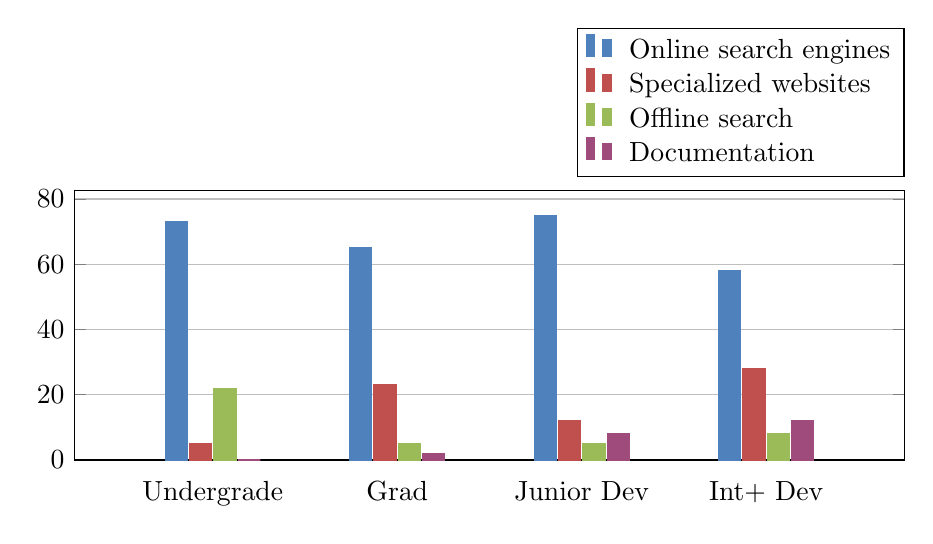
\begin{tikzpicture}
   \begin{axis}[
       width  = \textwidth,
       height = 5cm,
       major x tick style = transparent,
       ybar=2*\pgflinewidth,
       bar width=8pt,
       ymajorgrids = true,
       symbolic x coords={Undergrade, Grad, Junior Dev, Int+ Dev},
       xtick = data,
       scaled y ticks = false,
       enlarge x limits=0.25,
       ymin=0,
       legend cell align=left,
       legend style={
               at={(1,1.05)},
               anchor=south east,
               column sep=1ex
       }
   ]
       \addplot[style={bblue,fill=bblue,mark=none}]
           coordinates {(Undergrade, 73) (Grad,65) (Junior Dev,75) (Int+ Dev,58)};

       \addplot[style={rred,fill=rred,mark=none}]
             coordinates {(Undergrade, 5) (Grad,23) (Junior Dev,12) (Int+ Dev,28)};

       \addplot[style={ggreen,fill=ggreen,mark=none}]
             coordinates {(Undergrade, 22) (Grad,5) (Junior Dev,5) (Int+ Dev,8)};

       \addplot[style={ppurple,fill=ppurple,mark=none}]
           coordinates {(Undergrade, 0) (Grad,2) (Junior Dev,8) (Int+ Dev,12)};

       \legend{Online search engines, Specialized websites, Offline search , Documentation}
   \end{axis}
\end{tikzpicture}

    \caption{Answers to \textit{When facing an unknown bug, crash or exception, where do you look for informations ?} in percentage\label{fig:infos}}
\end{figure}



\end{frame}

\begin{frame}
\frametitle{What developers search for facing an unknow bug ?}


\begin{figure}[h!]
  \centering

  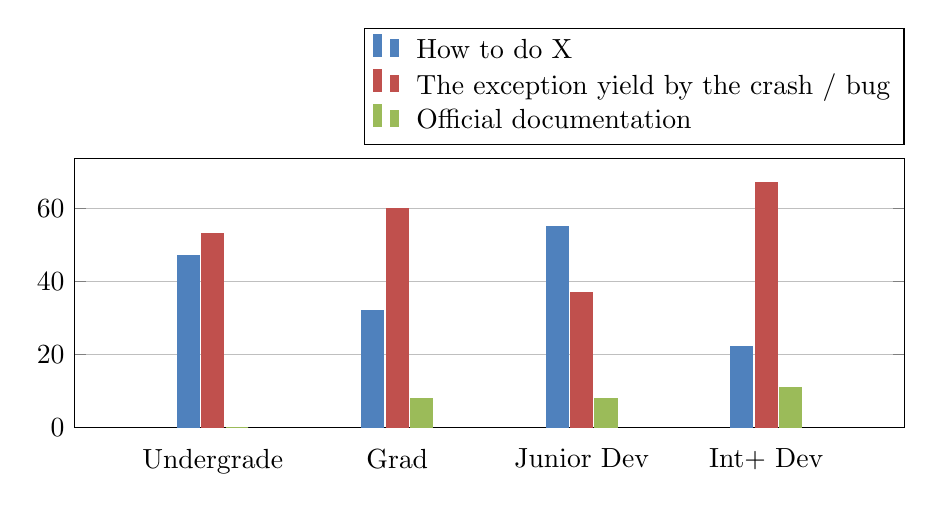
\begin{tikzpicture}
   \begin{axis}[
       width  = \textwidth,
       height = 5cm,
       major x tick style = transparent,
       ybar=2*\pgflinewidth,
       bar width=8pt,
       ymajorgrids = true,
       symbolic x coords={Undergrade, Grad, Junior Dev, Int+ Dev},
       xtick = data,
       scaled y ticks = false,
       enlarge x limits=0.25,
       ymin=0,
       legend cell align=left,
       legend style={
               at={(1,1.05)},
               anchor=south east,
               column sep=1ex
       }
   ]
       \addplot[style={bblue,fill=bblue,mark=none}]
           coordinates {(Undergrade, 47) (Grad,32) (Junior Dev,55) (Int+ Dev,22)};

       \addplot[style={rred,fill=rred,mark=none}]
             coordinates {(Undergrade, 53) (Grad,60) (Junior Dev,37) (Int+ Dev,67)};

       \addplot[style={ggreen,fill=ggreen,mark=none}]
             coordinates {(Undergrade, 0) (Grad,8) (Junior Dev,8) (Int+ Dev,11)};


       \legend{How to do X, The exception yield by the crash / bug, Official documentation}
   \end{axis}
\end{tikzpicture}
\end{figure}



\end{frame}

\begin{frame}

  \frametitle{BUMPER Data (as of now)}

  \begin{table}[]
  \centering
  \caption{
  RESOLVED/FIXED BUG (R/F BR),  CHANGESETS (CS), AND
  PROJECTS BY DATASET}
  \label{tab:summary}
  \begin{tabular}{c|c|c|c|c}
  \textbf{Dataset} & \textbf{R/F BR} & \textbf{CS} & \textbf{Files} & \textbf{Projects} \\ \hline \hline
  Gnome            & 550,869         & 1,231,354   & 367,245        & 512                \\ \hline
  Netbeans         & 53,258          & 122,632     & 30,595         & 39                \\ \hline
  Apache           & 49,449          & 106,366     & 38,111         & 349               \\ \hline
  Eclipse          & 78,830          & 184,900     & 21,712         & 190                \\ \hline \hline
  Total            & 732,406         & 1,645,252   & 457,663        & 1,930               \\ \hline \hline
  \end{tabular}
  \vspace{-2em}
  \end{table}

\end{frame}

\begin{frame}

  \frametitle{BUMPER Metamodel}

  \begin{figure*}
    \centering
    \includegraphics[width=0.9\textwidth]{../media/Bumper-Model.png}
  \vspace{-1.8em}
  \end{figure*}

\end{frame}

\begin{frame}

  \frametitle{BUMPER Use Cases}

\begin{itemize}
  \item Search for $"YOUR~TERMS"$ in bug reports and bug fix.
\end{itemize}

  \begin{equation*}
  \begin{split}
  ~~(type:``BUG"~AND~report\_t:``YOUR~TERMS"~~AND~-churns:0)\\
  ~~OR~\\
  ~~(\{!parent~which=``type:BUG"\}type:~\\
  ~~``CHANGESET"~AND~fix\_t:``YOUR~TERMS")
  \end{split}
  \end{equation*}

\end{frame}

\begin{frame}

  \frametitle{BUMPER Use Cases Cont'd}


  \begin{equation*}
  \begin{split}
    (type:``BUG"~AND~report_t:``Exception"~\\
  ~~AND~(project:``Axis2"~OR~project:``ide")~\\
  ~~AND~(reporter:``Rich"~OR~resolution:``fixed")~\\
  ~~AND~(severity:``Major"~OR~fixing\_time:[10~TO~*])~\\
  ~~AND~-churns:0)
  \end{split}
  \end{equation*}


\end{frame}

\begin{frame}

  \frametitle{Or ... you can let BUMPER find what your are looking for...}

  \begin{figure*}
    \centering
    \includegraphics[width=0.9\textwidth]{../media/interface.png}
  \vspace{-1.8em}
  \end{figure*}

\end{frame}

\begin{frame}

  \frametitle{Or ... you can let BUMPER find what your are looking for...}

  \begin{figure*}
    \centering
    \includegraphics[width=0.9\textwidth]{../media/interface2.png}
  \end{figure*}

\end{frame}


\begin{frame}

\frametitle{BUMPER}
\begin{itemize}
\item BUMPER: Bug Metarepository Search Engine for Developers and Researchers
\begin{itemize}
\item Online Search Engine with 1 million bug reports AND fixes from major open-source repositories
\item Apache Software Foundation, Netbeans, Eclipse, Gnome, FireFox, Chrome, Kde, ...
\item Imports bugs reports from Bugzilla, JIRA and Github, ... and fixes from SVN, Mercurial, Git, ...
\item Natural language for developers
\item Advanced API for researchers
\end{itemize}

\end{itemize}

\end{frame}

\begin{frame}
\frametitle{Conclusion and Future work}

\begin{itemize}
\item https://bumper-app.com
\item 1 million bugs and associated fixes
\item Apache Software Foundation, Netbeans, Eclipse, Gnome, FireFox, Chrome, Kde, ...
\item Imports bugs from Bugzilla, JIRA and Github, ... and fixes from SVN, Mercurial, Git, ...
\item Natural Language Search for developers
\item Advanced API for researchers
\vspace{0.5cm}
\item Currently assessing how much faster a suitable solution can be found using BUMPER rather than Google/Stack Overflow/Books ...
\end{itemize}



\end{frame}

%------------------------------------------------


%------------------------------------------------

\begin{frame}
\Huge{\centerline{QUESTIONS?}}
\end{frame}

%----------------------------------------------------------------------------------------

\end{document}
